\documentclass{article}
\usepackage{geometry}
\geometry{
	a4paper,
	total={170mm,257mm},
	left=20mm,
	top=20mm,
}
\usepackage{amsmath}
\usepackage{amssymb}
\usepackage{graphicx}
\usepackage{subcaption}
\graphicspath{ {./images/} }
\usepackage[utf8]{inputenc}
\usepackage{epigraph}
\usepackage{listings}
\title{QF603 Behavior Finance}
\date{Nov 24th 2018}
\author{Xia Xicheng}

\begin{document}
	\maketitle

\section{Behavioral Finance}


\begin{figure}[h]
	\centering
	\begin{subfigure}[b]{0.45\textwidth}
		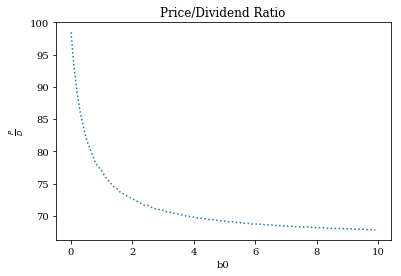
\includegraphics[width=\textwidth]{output_9_0.png}
		\caption{Price/Dividend Ratio}
		\label{fig:pd_ratio}
	\end{subfigure}
	~ %add desired spacing between images, e. g. ~, \quad, \qquad, \hfill etc. 
	%(or a blank line to force the subfigure onto a new line)
	\begin{subfigure}[b]{0.45\textwidth}
		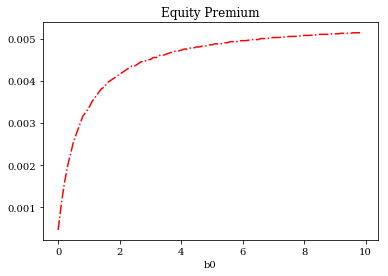
\includegraphics[width=\textwidth]{output_9_1.png}
		\caption{Equity Premium}
		\label{fig:ep}
	\end{subfigure}
	\caption{}\label{fig:ts_PL}
\end{figure}

\begin{itemize}
	\item The function calculate utility directly from the summation of the utility of comsumption and utility of recent financial gain or loss without a pricing kernel.
	
	\item  b0 measures the degree of prospect effect. A higher b0 means more impact of previous financial gain or loss on investor's utility (relative to consumption), which shows on the figures as higher euity premium and lower price/divident (more fruits) ratio.
	
	\item  $\lambda$ measures the degree of loss reversion. $\lambda$ larger than 1 means one loss more satisfaction when suffering from certain amount of loss compared to gain the same amount of profit.
\end{itemize}

\section{Python Code}
\begin{lstlisting}[language=Python, caption=Python Code]
import numpy as np
import pandas as pd
import matplotlib.pyplot as plt

plt.rcParams['font.family'] = 'serif'
plt.rcParams['figure.facecolor'] = '1.'

# lock the random
np.random.seed(1)

# simulate epsilon
epsilon = np.random.randn(10000, 1)

# calculate ln(g)
ln_g = 0.02 + 0.02 * epsilon

# calculate g
g = np.exp(ln_g)

plt.plot(g)
plt.title('g')
plt.show()

M = 0.99 * g**(-1)

PD = np.mean( 0.99*g**(1 - 1) )

def e(x, b0, lambd = 2): 

	def v(array):
		ind0 = array >= 1.0303
		ind1 = array < 1.0303
		
		value = np.zeros(array.shape)
		value[ind0] = array[ind0] - 1.0303
		value[ind1] = lambd*( array[ind1] - 1.0303 )
		
		return value
	
	error = 0.99*b0*( np.mean(v(x*g)) ) + 0.99*x - 1
	
	return error

def bisection_search(function, guess_minus, guess_plus):
	'''Bisection search optimization
	Find out the x_ that makes function(x_) appoaximate to 0 (1e-4).
	*function* must be continuous. 
	*function(guess_minus)* and *function(guess_plus)* must have opposite signs.
	
	Input:
	--- function: The objective function to be optimized.
	fun(x, *args) -> 0
	
	--- guess_minus: One end of the bracketing interval [x-, x+].
	float or integer
	
	--- guess_plus: One end of the bracketing interval [x-, x+].
	float or integer
	
	Output:
	--- x_: optimal x that satisfies fun(x, *args) -> 0
	float
	'''
	# guarantee the optimal x is in [x-, x+]
	assert function(guess_minus)*function(guess_plus)<0,\
	'*function(guess_minus)* and *function(guess_plus)* must be sign changing values'
	
	# switch the position if the negative and positive bound are reversed
	if function(guess_minus) > 0:
		guess_minus,  guess_plus = guess_plus, guess_minus
	
	# assign the current optimal guess to x_
	if abs( function(guess_minus) ) > abs( function(guess_plus) ):
		x_ = guess_plus
	else:
		x_ = guess_minus
	
	# optimization goal is 1e-4
	while abs( function(x_) ) > 1e-4:
		# take the midpoint as new bound.
		x_ = (guess_plus + guess_minus)/2
		
		# update guess_plus/guess_minus
		if function(x_) > 0:
			guess_plus = x_ 
		else:
			guess_minus = x_
	
	return x_

b_array = np.arange(0, 10, 0.1)

x_array = np.array( [bisection_search(lambda x, b0 = b: e(x, b0), 1., 1.1 ) for b in b_array ] )

PD_array = np.array( [1/(x - 1) for x in x_array] )

ERM_array = np.array( [np.mean(x*g) for x in x_array] )

Rf = 1/np.mean(0.99*g**(- 1))

plt.plot(b_array, PD_array, ':' )
plt.title('Price/Dividend Ratio')
plt.xlabel('b0')
plt.ylabel('$\\frac{P}{D}$')
plt.show()

plt.plot( b_array, ERM_array - Rf, 'r-.' )
plt.title('Equity Premium')
plt.xlabel('b0')
plt.show()
\end{lstlisting}

\end{document}